\documentclass[11pt]{article} 
\usepackage[english]{babel}
\usepackage[utf8]{inputenc}
\usepackage[margin=0.5in]{geometry}
\usepackage{amsmath}
\usepackage{amsthm}
\usepackage{amsfonts}
\usepackage{amssymb}
\usepackage[usenames,dvipsnames]{xcolor}
\usepackage{graphicx}
\usepackage[siunitx]{circuitikz}
\usepackage{tikz}
\usepackage{tkz-berge}
\usetikzlibrary{positioning, automata, backgrounds}
\usepackage[colorinlistoftodos, color=orange!50]{todonotes}
\usepackage{hyperref}
\usepackage[numbers, square]{natbib}
\usepackage{fancybox}
\usepackage{epsfig}
\usepackage{soul}
\usepackage[framemethod=tikz]{mdframed}
\usepackage[shortlabels]{enumitem}
\usepackage[version=4]{mhchem}
\usepackage{multicol}
\usepackage{forest}
\usepackage{mathtools}
\usepackage{comment}
\usepackage{enumitem}
\usepackage[utf8]{inputenc}
\usepackage[linesnumbered,ruled,vlined]{algorithm2e}
\usepackage{listings}
\usepackage{color}
\usepackage[numbers]{natbib}
\usepackage{subfiles}
\usepackage{tkz-berge}


\newtheorem{prop}{Proposition}[section]
\newtheorem{thm}{Theorem}[section]
\newtheorem{lemma}{Lemma}[section]
\newtheorem{cor}{Corollary}[prop]

\theoremstyle{definition}
\newtheorem{definition}{Definition}

\theoremstyle{definition}
\newtheorem{required}{Problem}

\theoremstyle{definition}
\newtheorem{ex}{Example}

\newcommand{\interval}[4]{\draw (#2, #1) -- (#3, #1); % Usage: \interval{height}{start}{end}{label}
\draw (#2, #1-0.11) -- (#2, #1+0.11); % draw left whisker
\draw (#3, #1-0.11) -- (#3, #1+0.11); % draw right whisker
\node[] at (#2-0.6, #1) {#4};
}
\newcommand{\floor}[1]{\lfloor #1 \rfloor}
\def\checkmark{\tikz\fill[scale=0.4](0,.35) -- (.25,0) -- (1,.7) -- (.25,.15) -- cycle;}

\setlength{\marginparwidth}{3.4cm}
%#########################################################

%To use symbols for footnotes
\renewcommand*{\thefootnote}{\fnsymbol{footnote}}
%To change footnotes back to numbers uncomment the following line
%\renewcommand*{\thefootnote}{\arabic{footnote}}

% Enable this command to adjust line spacing for inline math equations.
% \everymath{\displaystyle}

% _______ _____ _______ _      ______ 
%|__   __|_   _|__   __| |    |  ____|
%   | |    | |    | |  | |    | |__   
%   | |    | |    | |  | |    |  __|  
%   | |   _| |_   | |  | |____| |____ 
%   |_|  |_____|  |_|  |______|______|
%%%%%%%%%%%%%%%%%%%%%%%%%%%%%%%%%%%%%%%

\title{
\normalfont \normalsize 
\textsc{CSCI 3104 Summer 2021 \\ 
Instructor: Michael Levet} \\
[10pt] 
\rule{\linewidth}{0.5pt} \\[6pt] 
\huge Problem Set 4 \\
\rule{\linewidth}{2pt}  \\[10pt]
}
\author{Brian E. Peterson}
\date{06/16/2021}

\begin{document}

\maketitle


%%%%%%%%%%%%%%%%%%%%%%%%%
%%%%%%%%%%%%%%%%%%%%%%%%%%
%%%%%%%%%%Brian E. Peterson%%%%%%%
%%%%%%%%%%109067890%%%%%%%%
%%%%%%%%%%%%%%%%%%%%%%%%%%
\noindent
Due Date \dotfill 06/16/2021 \\
Name \dotfill \textbf{Brian E. Peterson} \\
Student ID \dotfill \textbf{109067890} \\
Collaborators \dotfill \textbf{N/A}

\tableofcontents

\section{Instructions}
 \begin{itemize}
	\item The solutions \textbf{must be typed}, using proper mathematical notation. We cannot accept hand-written solutions. \href{http://ece.uprm.edu/~caceros/latex/introduction.pdf}{Here's a short intro to \LaTeX.}
	\item You should submit your work through the \textbf{class Canvas page} only. Please submit one PDF file, compiled using this \LaTeX \ template.
	\item You may not need a full page for your solutions; pagebreaks are there to help Gradescope automatically find where each problem is. Even if you do not attempt every problem, please submit this document with no fewer pages than the blank template (or Gradescope has issues with it).

	\item You are welcome and encouraged to collaborate with your classmates, as well as consult outside resources. You must \textbf{cite your sources in this document.} \textbf{Copying from any source is an Honor Code violation. Furthermore, all submissions must be in your own words and reflect your understanding of the material.} If there is any confusion about this policy, it is your responsibility to clarify before the due date. 

	\item Posting to \textbf{any} service including, but not limited to Chegg, Reddit, StackExchange, etc., for help on an assignment is a violation of the Honor Code.

	\item You \textbf{must} virtually sign the Honor Code (see Section \ref{HonorCode}). Failure to do so will result in your assignment not being graded.
\end{itemize}


\section{Honor Code (Make Sure to Virtually Sign the Honor Pledge)} \label{HonorCode}

\begin{required}
On my honor, my submission reflects the following:
\begin{itemize}
\item My submission is in my own words and reflects my understanding of the material.
\item Any collaborations and external sources have been clearly cited in this document.
\item I have not posted to external services including, but not limited to Chegg, Reddit, StackExchange, etc.
\item I have neither copied nor provided others solutions they can copy.
\end{itemize}

\noindent In the specified region below, clearly indicate that you have upheld the Honor Code. Then type your name. 
\end{required}

\begin{proof}[Honor Pledge]
\begin{itemize}
	\item My submission is in my own words and reflects my understanding of the material.
	\item Any collaborations and external sources have been clearly cited in this document.
	\item I have not posted to external services including, but not limited to Chegg, Reddit, StackExchange, etc.
	\item I have neither copied nor provided others solutions they can copy.
\end{itemize}
Brian E. Peterson
\end{proof}


\newpage
\section{Standard 4- Examples Where Greedy Algorithms Fail}

\subsection{Problem \ref{GreedyFail1}}
\begin{required} \label{GreedyFail1}
Recall the \textsf{Interval Scheduling} problem, where we take as input a set of intervals $\mathcal{I}$. The goal is to find a maximum-sized set $S \subseteq \mathcal{I}$, where no two intervals in $S$ intersect. Consider the greedy algorithm where we place all of the intervals of $\mathcal{I}$ into a priority queue, ordered earliest start time to latest start time. We then construct a set $S$ by adding intervals to $S$ as we poll them from the priority queue, provided the element we polled does not intersect with any interval already in $S$. \\

\noindent Provide an example with at least $5$ intervals where this algorithm fails to yield a maximum-sized set of pairwise non-overlapping intervals. Clearly specify both the set $S$ that the algorithm constructs, as well a larger set of pairwise non-overlapping intervals. \\

\noindent You may explicitly specify the intervals by their start and end times (such as in Example 35 of the course notes) or by drawing them. You are welcome to hand-draw and embed an image, provided it is legible and we do not have to rotate our screens to grade your work. Your justification should still be typed. If you would prefer to draw the intervals using \LaTeX, we have provided sample code below.
\end{required}

\begin{proof}[Answer]

\begin{tikzpicture}[thick, framed]   
	\interval{3.3}{1}{3}{A}
	\interval{2.6}{2.5}{3.5}{B}
	\interval{1.9}{1}{2}{C}
	\interval{1.2}{4}{6}{D}
	\interval{0.5}{7}{9}{E}
\end{tikzpicture}

Given this set of intervals, $\mathcal{I}$, the above described algorithm would construct the following set, $S$:
\[
	[A, D, E]	
\]
The algorithm would construct this set because A and C have the same start time, but A appears first. If we assume
the priority queue would contain first $A$, then $C$, followed by $B$, $D$, and $E$, then the initial choice of $A$ would result
in not including 2 intervals which could be exchanged for $A$, thus finding a non-maximum-sized set. However, the maximum-sized set of pairwise non-overlapping intervals would actually be:
\[
	[C, B, D, E]
\]

\end{proof}

\newpage
\subsection{Problem \ref{GreedyFail2}}
\begin{required} \label{GreedyFail2}
Recall that the length of an interval $[s, f]$ is $f - s$. Consider a greedy algorithm which works identically as in Problem \ref{GreedyFail1}, except we sort the intervals from longest to shortest. Draw an example with at least 5 appointments where this algorithm fails. Show the order in which the algorithm selects the intervals, and also show a larger subset of non-overlapping intervals than the subset output by the greedy algorithm. The same comments apply here as for Problem \ref{GreedyFail1} in terms of level of explanation.
\end{required}

\begin{proof}[Answer]

Take this set of intervals, $\mathcal{I}$:

\begin{tikzpicture}[thick, framed]   
	\interval{3.3}{1}{9}{A}
	\interval{2.6}{2}{3}{B}
	\interval{1.9}{3.5}{5}{C}
	\interval{1.2}{5.5}{6.5}{D}
	\interval{0.5}{7}{8.5}{E}
\end{tikzpicture}

The algorithm would first produce this ordering:
\[
	[A, C, E, B, D]
\]
Then it would put $A$ into $S$ and then immediately terminate, because all other intervals intersect with $A$,
and $A$ was selected first, precluding adding any more intervals. Yielding a final set $S$:

\[ 
	[A]
\] 

This is clearly not the maximum-sized set of intervals in $\mathcal{I}$, which is actually (leaving the sort order as above):

\[
	[C, E, B, D]	
\]

\end{proof}

\newpage
\subsection{Problem \ref{GreedyFail3}}
\begin{required} \label{GreedyFail3}
Consider now the \textsf{Weighted Interval Scheduling} problem, where each interval $i$ is specified by 
\[
([\text{start}_{i}, \text{end}_{i}], \text{weight}_{i}). 
\]

\noindent Here, the weight is an assigned value that is independent of the length $\text{end}_{i} - \text{start}_{i}$. Here, you may assume $\text{weight}_{i} > 0$. We seek a set $S$ of pairwise non-overlapping intervals that maximizes $\sum_{i \in S} \text{weight}_{i}$. That is, rather than maximizing the number of intervals, we are seeking to maximize the sum of the weights. \\

\noindent Consider a greedy algorithm which works identically as in Problem \ref{GreedyFail1}. Draw an example with at least 5 appointments where this algorithm fails. Show the order in which the algorithm selects the intervals, and also show a subset with larger weight of non-overlapping intervals than the subset output by the greedy algorithm. The same comments apply here as for Problem \ref{GreedyFail1} in terms of level of explanation.
\end{required}

\begin{proof}[Answer]

	Consider this example:
	
	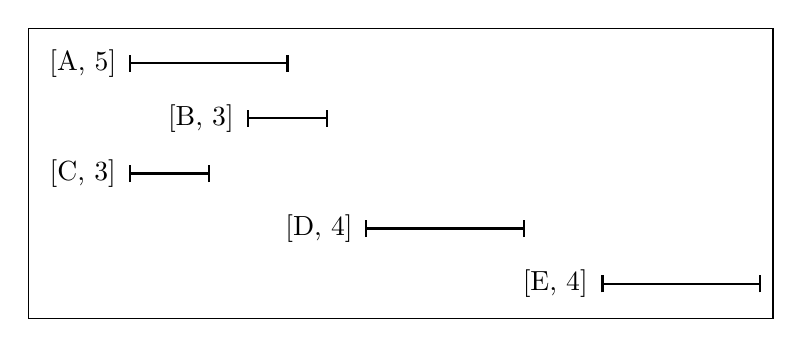
\begin{tikzpicture}[thick, framed]   
		\interval{3.3}{1}{3}{[A, 5]}
		\interval{2.6}{2.5}{3.5}{[B, 3]}
		\interval{1.9}{1}{2}{[C, 3]}
		\interval{1.2}{4}{6}{[D, 4]}
		\interval{0.5}{7}{9}{[E, 4]}
	\end{tikzpicture}

	Let the weight of each interval be the number which follows the interval's label, e.g. $[F, 6]$ has weight $6$. 
	This is notably, essentially the same answer I gave for \ref{GreedyFail1}. Again, the algorithm sorts these as follows (by start time, not weight -- this is the problem specification):
	\[
		[A, C, B, D, E]	
	\] 
	Upon polling $A$, then $C$ and $B$ become inadmissible into $S$ because they intersect with $A$. Adding $D$ and $E$,
	this yields:
	\[
		[A, D, E]
	\]
	However, this has weights $5+4+4 = 13$, whereas the set of intervals with maximum weights is:
	\[
		[C, B, D, E],
	\]
	Having weights $3+3+4+4 = 14$.

\end{proof}



\newpage
\section{Standard 5- Exchange Arguments}

\subsection{Problem \ref{Exchange1}}
\begin{required} \label{Exchange1}
Recall the Making Change problem, where we have an infinite supply of pennies (worth $1$ cent), nickels (worth $5$ cents), dimes (worth $10$ cents), and quarters (worth $25$ cents). We take as input an integer $n \geq 0$. The goal is to make change for $n$ using the fewest number of coins possible. \\

\noindent Prove that in an optimal solution, we use at most $4$ pennies.
\end{required}

\begin{proof}

Let $S$ be the multiset of coins, with which, we wish to make change for $n$. Suppose $S$ contains $k > 4$ pennies, so $k \geq 5$. By the division algorithm,
\[
	k = 5j + r
\]
For $k > 4$, we can exchange $j$, or $\floor{\dfrac{k}{5}}$, quintets of pennies for $1$ nickel.
This results in $4j$ fewer coins needed to make change for n, as we remove $5$ pennies while adding $1$ nickel, for each exchange that we make. If $k > 4$, we can make at least
one such exchange, since $j > 0$. Therefore, in an optimal change-making solution, we will use at most $4$ pennies because we will have made all possible such exchanges which can each 
remove 4 coins from our total solution, i.e. our solution will have the minimal number of coins (and also the minimum).
\end{proof}



\newpage
\subsection{Problem \ref{Exchange2}}

\begin{required} \label{Exchange2}
Consider the \textsf{Interval Projection} problem, which is defined as follows.
\begin{itemize}
\item \textsf{Instance:} Let $\mathcal{I}$ be a set of intervals on the real line.
\item \textsf{Solution:} A minimum sized set $S$ of points on the real line, such that (i) for every interval $[s, f] \in \mathcal{I}$, there exists a point $x \in S$ where $x$ is in the interval $[s, f]$. We call $S$ a \textit{projection set}.
\end{itemize}

\noindent Do the following.
\begin{enumerate}[label=(\alph*)]
\subsubsection{Problem 6\ref{6a}}
\item \label{6a} Find a minimum sized projection set $S$ for the following set of intervals:
\begin{align*}
\mathcal{I} = \{ [0, 1], [0.5, 1], [1, 1.5], [1.4, 2], [1.6, 2.3] \}.
\end{align*}


\begin{proof}[Answer]
\[
	S = \{ 0.5, 1.4, 2.3 \}	
\]
This is a projection set for $\mathcal{I}$ because $0.5$ is in both of the first two intervals, $1.4$ is contained in the third and fourth, and 2.3 is contained in 
the last. It's a minimal-sized projection set because any point in $[0.5, 1]$ satisfies the first two intervals (this is their intersection), any point in $[1.4, 1.5]$ satisfies the third and fourth intervals (again, their intersection), and any point in $[1.6, 2.3]$ satisfies the last interval (no change made).
However, these intersections of the original intervals are pairwise non-overlapping, and thus no less than $3$ points, $1$ for each interval, can serve as a projection set for them. This is the size of our given solution, so we do have a minimum-sized projection set. 

\end{proof}

\newpage
\subsubsection{Problem 6\ref{6b}}
\item \label{6b} Fix a set of intervals $\mathcal{I}$, and let $S$ be a projection set. Prove that there exists a projection set $S^{\prime}$ where every point $x \in S^{\prime}$ is the right end-point of interval $[s, f] \in \mathcal{I}$. 

\begin{proof}

\textbf{Base case}. Consider the case when $\mathcal{I} = \{\}$. 

By definition, a projection set $S$ is a set of points on the real line, 
such that for every interval $[s, f] \in \mathcal{I}$, 
there exists a point $x \in S$ where $x$ is in the interval $[s, f]$.

In the case of $\mathcal{I} = \{\}$ (the empty set), the only valid projection set is by definition also the empty set.
This is indeed a projection set, because for each interval in $\mathcal{I}$, (i.e. no intervals),
there exists a point. Because the premise never holds (there are no intervals), the proposition is always true 
(there exists a point for each non-existent interval).

For a similar reason, this projection set is also one where every point $x \in S^{\prime}$ is the right end-point of an interval,
i.e. there are no points, and all of them (none) are right end-points of intervals in $\mathcal{I}$.  \checkmark

\textbf{Inductive hypothesis}. Fix $k > 0$. Assume for $|\mathcal{I}| = k$, there is a projection set $S^{\prime}$ where every point $x \in S^{\prime}$ is the right end-point of one of the $k$ intervals in $\mathcal{I}$.  

\textbf{Inductive step}. Consider the $k+1$st case.

From the inductive hypothesis (IH), we know there is some set of points, $S^{\prime}$, where every point is a right end-point of an interval from $\mathcal{I}$, and that this constitutes a projection set for $\mathcal{I}$.

Therefore, we know that all intervals except one new one, just added, are already "represented", and only by their or other right end-points, in some set, $S^{\prime}$.

Consider the case where the new interval is entirely contained within another, already "represented" interval. Then we already have a projection set which is valid for the $k+1$st case. Without adding any more points, we also know that every point in $S^{\prime}$ corresponds to the right end-point of some interval. \checkmark

Consider the case where the interval is not entirely contained within another, already "represented" interval. Then either the right or left or both end-points are outside all of our intervals. 

If only the left end-point is outside of our existing intervals, then the right end-point is inside our existing intervals. In this case, we again already have what we need: a representative point for our projection set which is the right end-point of an interval. \checkmark

If the right end-point is outside our existing intervals, we need to show that there is some new projection set $S^{\prime\prime}$ which can contain all the points in $S^{\prime}$, plus our new right endpoint.

Suppose the new interval being added to our $\mathcal{I}$ is $[s_i, f_i]$. Then, $S^{\prime\prime} = S^{\prime} \cup {f_i}$.

Therefore, by induction on $|\mathcal{I}|$, there always exists a projection set $S^{\prime}$ for $\mathcal{I}$, where every point $x \in S^{\prime}$ is the right end-point of some interval $[s, f] \in \mathcal{I}$.

\end{proof}

\end{enumerate}
\end{required}

\end{document} % NOTHING AFTER THIS LINE IS PART OF THE DOCUMENT



